\begin{center}
\large\noindent\fbox{
	\parbox{\textwidth}{
	  Utilizzare il metodo di Jacobi per risolvere il sistema lineare
	  $$
	  A_n \textbf{x} = \begin{pmatrix} 1 \\ \vdots \\ 1 \end{pmatrix}
	  $$

	  dove $A_n$ è la matrice definita nell'Esercizio 6.1, con tolleranza $tol=10^{-5}$, e partendo dal vettore nullo. Graficare il numero di iterazioni necessarie, rispetto alla dimensione $n$ del problema, con $n$ che varia da 100 a 1000 (con passo 20).
}
}\end{center}

\noindent Di seguito si riportano i codici Matlab utilizzati. La funzione di \textit{Jacobi} oltre ad effettuare il calcolo del vettore delle incognite della matrice $A$, restituisce anche il numero di iterazioni \textit{numIt} impiegate e la norma infinito del residuo, al passo i-simo.

\lstinputlisting[language=Matlab]{Codici/Cap6/SoluzioneEs3_Cap6.m}
\vspace*{0.5cm}
\lstinputlisting[language=Matlab]{Codici/Cap6/jacobi.m}
\vspace*{1cm}
\noindent Graficamente si pu\'o osservare il seguente risultato, al variare di \textit{n}: 

\begin{figure}[H]
	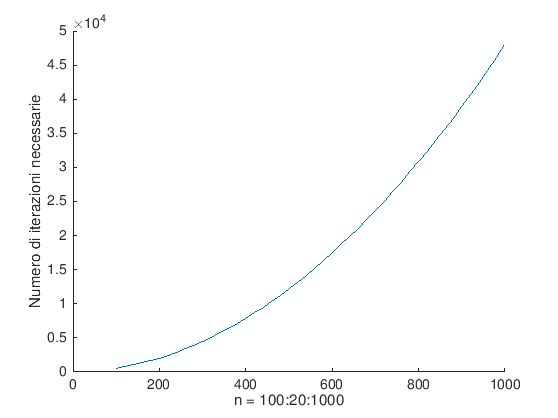
\includegraphics[width=\textwidth]{Codici/Cap6/es3_cap6}
\end{figure}